\PassOptionsToPackage{unicode=true}{hyperref} % options for packages loaded elsewhere
\PassOptionsToPackage{hyphens}{url}
%
\documentclass[ignorenonframetext,]{beamer}
\usepackage{pgfpages}
\setbeamertemplate{caption}[numbered]
\setbeamertemplate{caption label separator}{: }
\setbeamercolor{caption name}{fg=normal text.fg}
\beamertemplatenavigationsymbolsempty
% Prevent slide breaks in the middle of a paragraph:
\widowpenalties 1 10000
\raggedbottom
\setbeamertemplate{part page}{
\centering
\begin{beamercolorbox}[sep=16pt,center]{part title}
  \usebeamerfont{part title}\insertpart\par
\end{beamercolorbox}
}
\setbeamertemplate{section page}{
\centering
\begin{beamercolorbox}[sep=12pt,center]{part title}
  \usebeamerfont{section title}\insertsection\par
\end{beamercolorbox}
}
\setbeamertemplate{subsection page}{
\centering
\begin{beamercolorbox}[sep=8pt,center]{part title}
  \usebeamerfont{subsection title}\insertsubsection\par
\end{beamercolorbox}
}
\AtBeginPart{
  \frame{\partpage}
}
\AtBeginSection{
  \ifbibliography
  \else
    \frame{\sectionpage}
  \fi
}
\AtBeginSubsection{
  \frame{\subsectionpage}
}
\usepackage{lmodern}
\usepackage{amssymb,amsmath}
\usepackage{ifxetex,ifluatex}
\usepackage{fixltx2e} % provides \textsubscript
\ifnum 0\ifxetex 1\fi\ifluatex 1\fi=0 % if pdftex
  \usepackage[T1]{fontenc}
  \usepackage[utf8]{inputenc}
  \usepackage{textcomp} % provides euro and other symbols
\else % if luatex or xelatex
  \usepackage{unicode-math}
  \defaultfontfeatures{Ligatures=TeX,Scale=MatchLowercase}
\fi
% use upquote if available, for straight quotes in verbatim environments
\IfFileExists{upquote.sty}{\usepackage{upquote}}{}
% use microtype if available
\IfFileExists{microtype.sty}{%
\usepackage[]{microtype}
\UseMicrotypeSet[protrusion]{basicmath} % disable protrusion for tt fonts
}{}
\IfFileExists{parskip.sty}{%
\usepackage{parskip}
}{% else
\setlength{\parindent}{0pt}
\setlength{\parskip}{6pt plus 2pt minus 1pt}
}
\usepackage{hyperref}
\hypersetup{
            pdftitle={Regression with many features},
            pdfborder={0 0 0},
            breaklinks=true}
\urlstyle{same}  % don't use monospace font for urls
\newif\ifbibliography
\setlength{\emergencystretch}{3em}  % prevent overfull lines
\providecommand{\tightlist}{%
  \setlength{\itemsep}{0pt}\setlength{\parskip}{0pt}}
\setcounter{secnumdepth}{0}

% set default figure placement to htbp
\makeatletter
\def\fps@figure{htbp}
\makeatother


\title{Regression with many features}
\author{}
\date{\vspace{-2.5em}}

\begin{document}
\frame{\titlepage}

\begin{frame}{plot of chunk unnamed-chunk-2}
\protect\hypertarget{plot-of-chunk-unnamed-chunk-2}{}

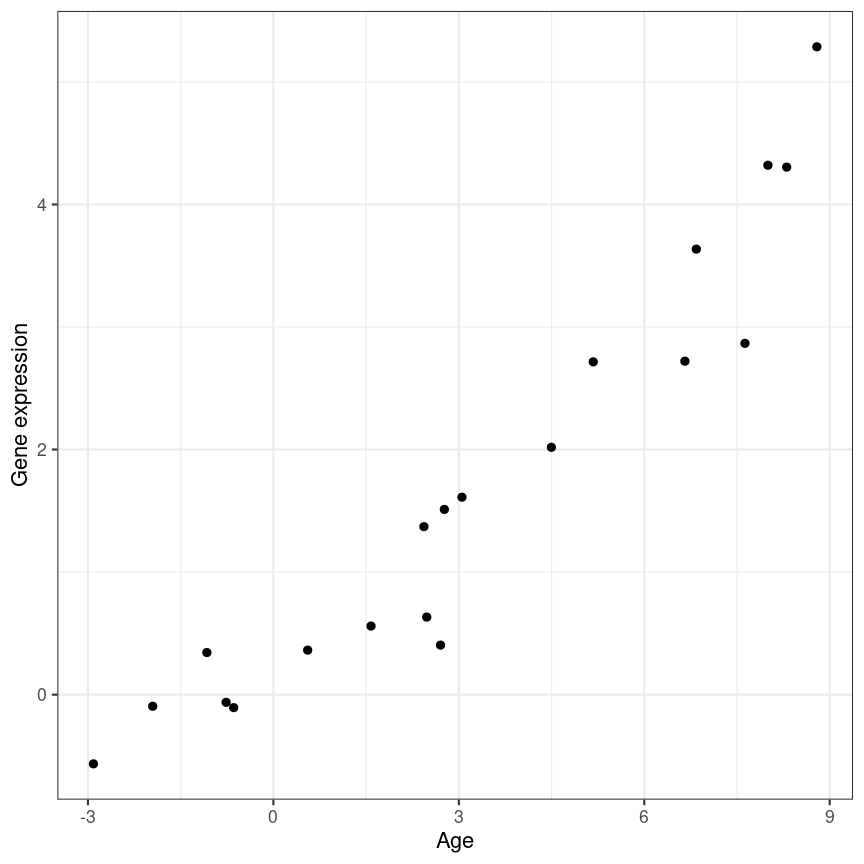
\includegraphics[width=0.5\textwidth]{/home/runner/work/high-dimensional-stats-r/high-dimensional-stats-r/fig/rmd-02-unnamed-chunk-2-1}



\end{frame}

\begin{frame}{plot of chunk unnamed-chunk-3}
\protect\hypertarget{plot-of-chunk-unnamed-chunk-3}{}

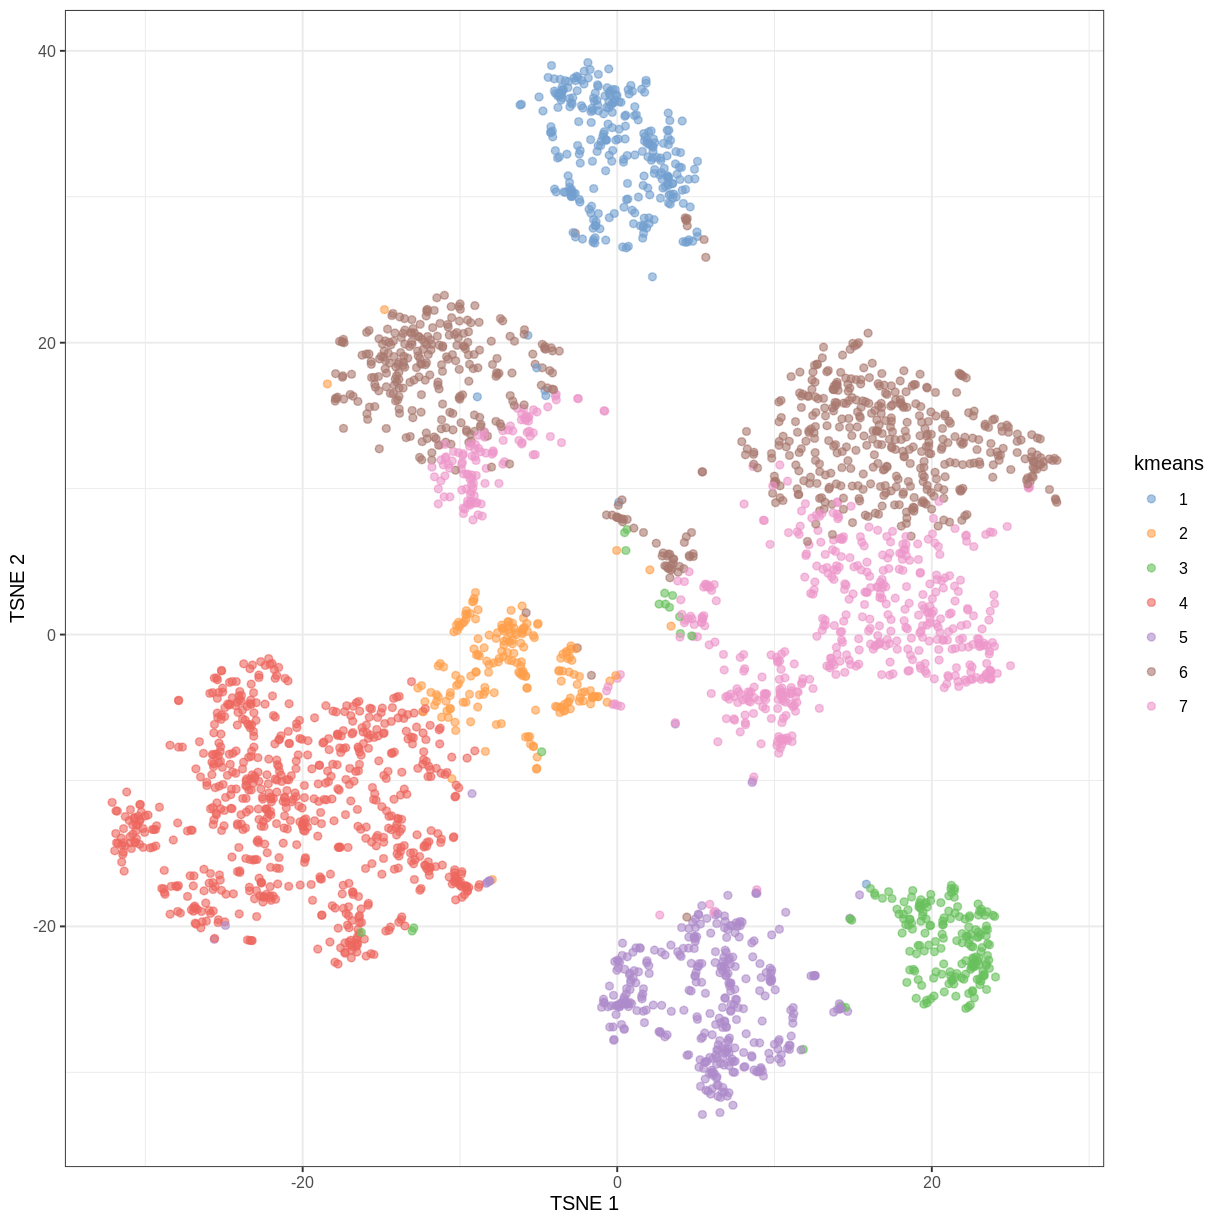
\includegraphics[width=0.5\textwidth]{/home/runner/work/high-dimensional-stats-r/high-dimensional-stats-r/fig/rmd-02-unnamed-chunk-3-1}



\end{frame}

\begin{frame}{plot of chunk unnamed-chunk-4}
\protect\hypertarget{plot-of-chunk-unnamed-chunk-4}{}

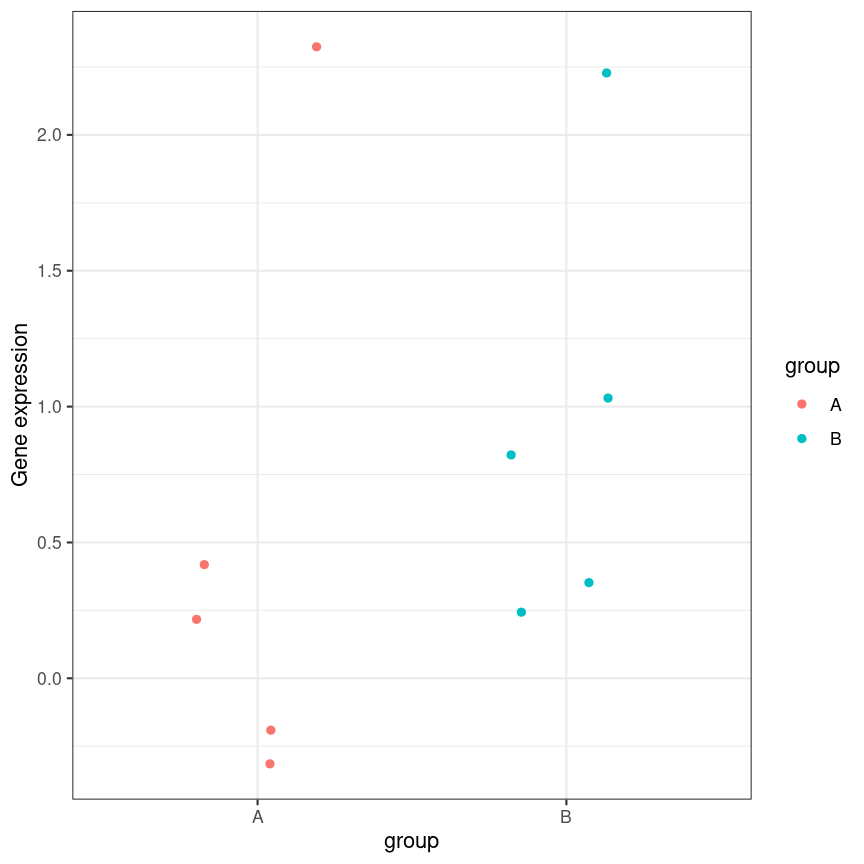
\includegraphics[width=0.5\textwidth]{/home/runner/work/high-dimensional-stats-r/high-dimensional-stats-r/fig/rmd-02-unnamed-chunk-4-1}



\end{frame}

\begin{frame}{plot of chunk unnamed-chunk-5}
\protect\hypertarget{plot-of-chunk-unnamed-chunk-5}{}

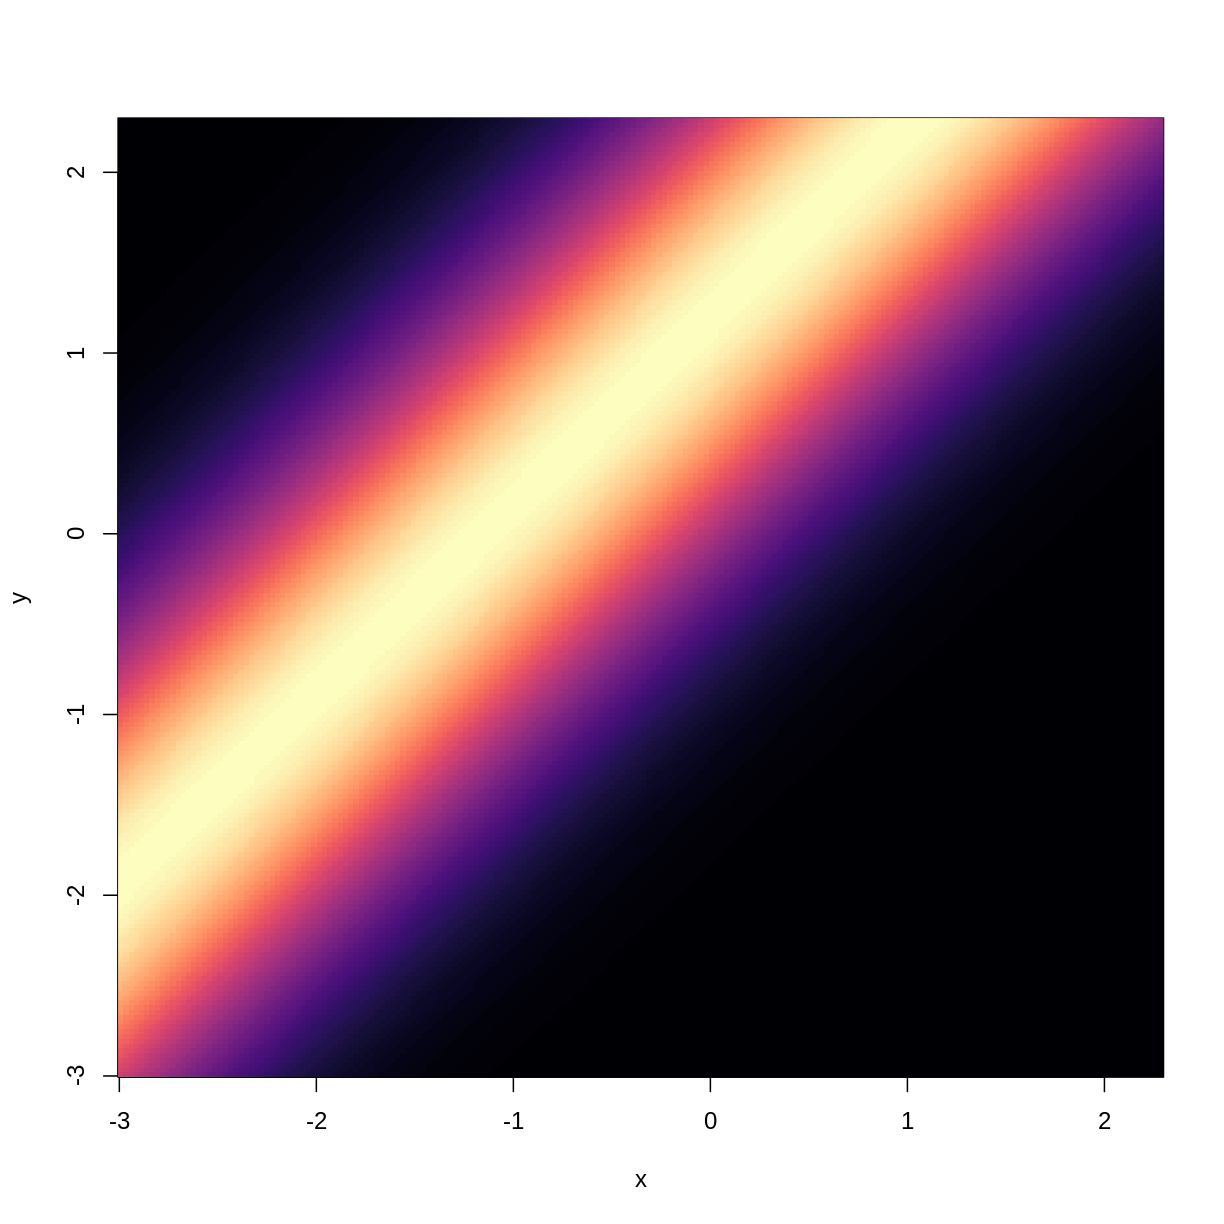
\includegraphics[width=0.5\textwidth]{/home/runner/work/high-dimensional-stats-r/high-dimensional-stats-r/fig/rmd-02-unnamed-chunk-5-1}



\end{frame}

\begin{frame}{Density plot of a t-distribution showing the observed test
statistics (here, t-statistics). The p-values, visualised here with
shaded regions, represent the portion of the null distribution that is
as extreme or more extreme as the observed test statistics, which are
shown as dashed lines.}
\protect\hypertarget{density-plot-of-a-t-distribution-showing-the-observed-test-statistics-here-t-statistics.-the-p-values-visualised-here-with-shaded-regions-represent-the-portion-of-the-null-distribution-that-is-as-extreme-or-more-extreme-as-the-observed-test-statistics-which-are-shown-as-dashed-lines.}{}

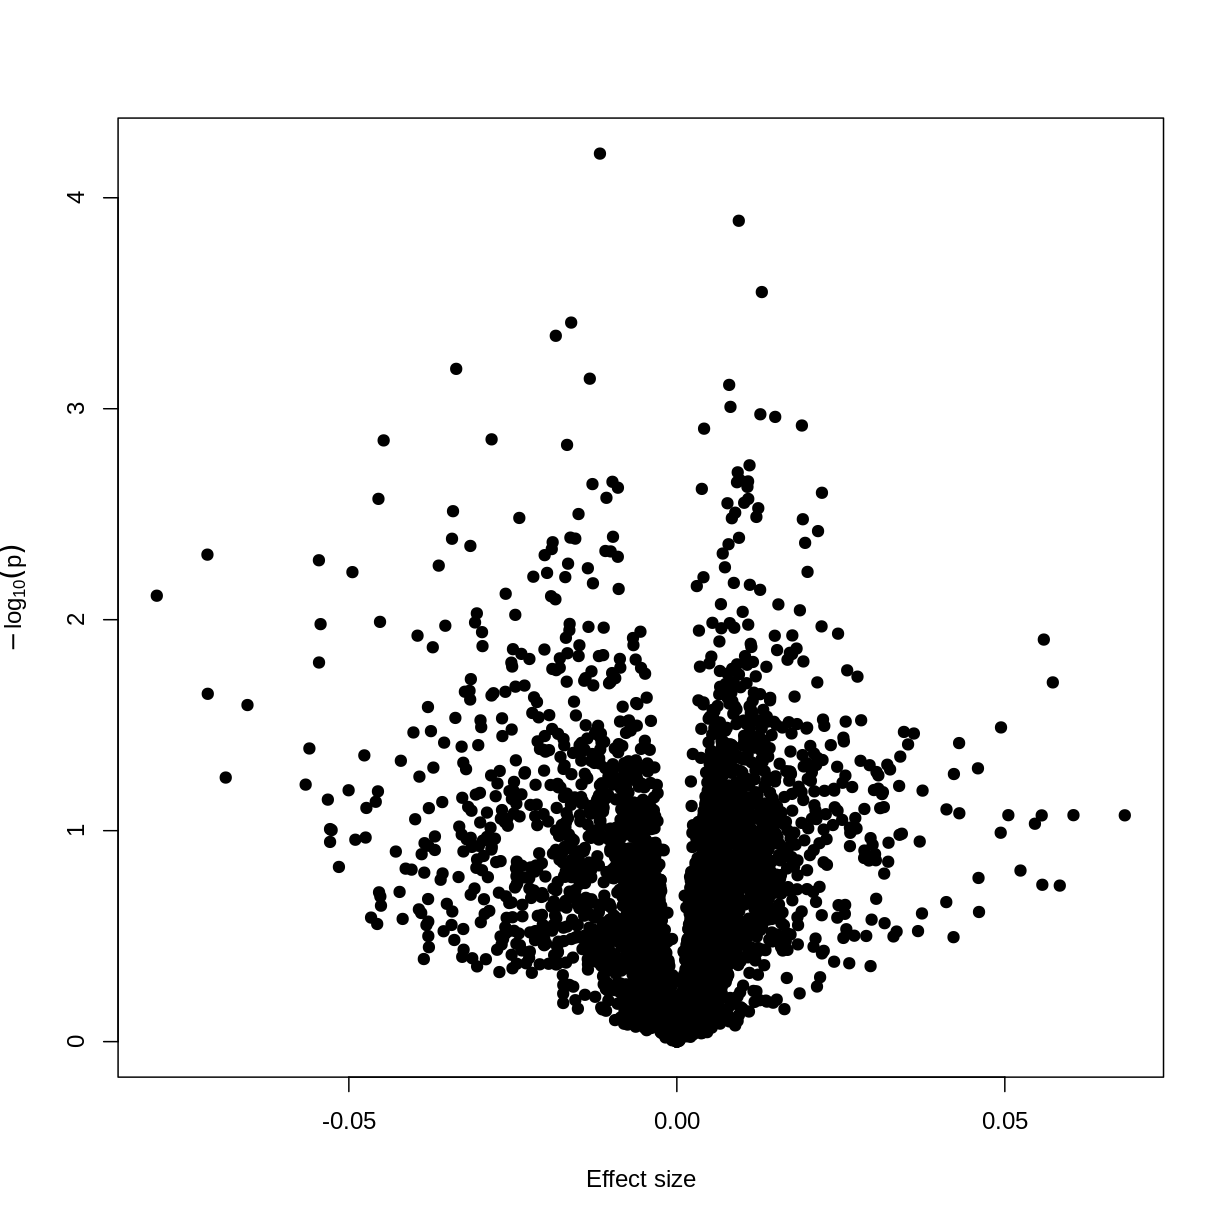
\includegraphics[width=0.5\textwidth]{/home/runner/work/high-dimensional-stats-r/high-dimensional-stats-r/fig/rmd-02-unnamed-chunk-8-1}



\end{frame}

\begin{frame}{plot of chunk unnamed-chunk-9}
\protect\hypertarget{plot-of-chunk-unnamed-chunk-9}{}

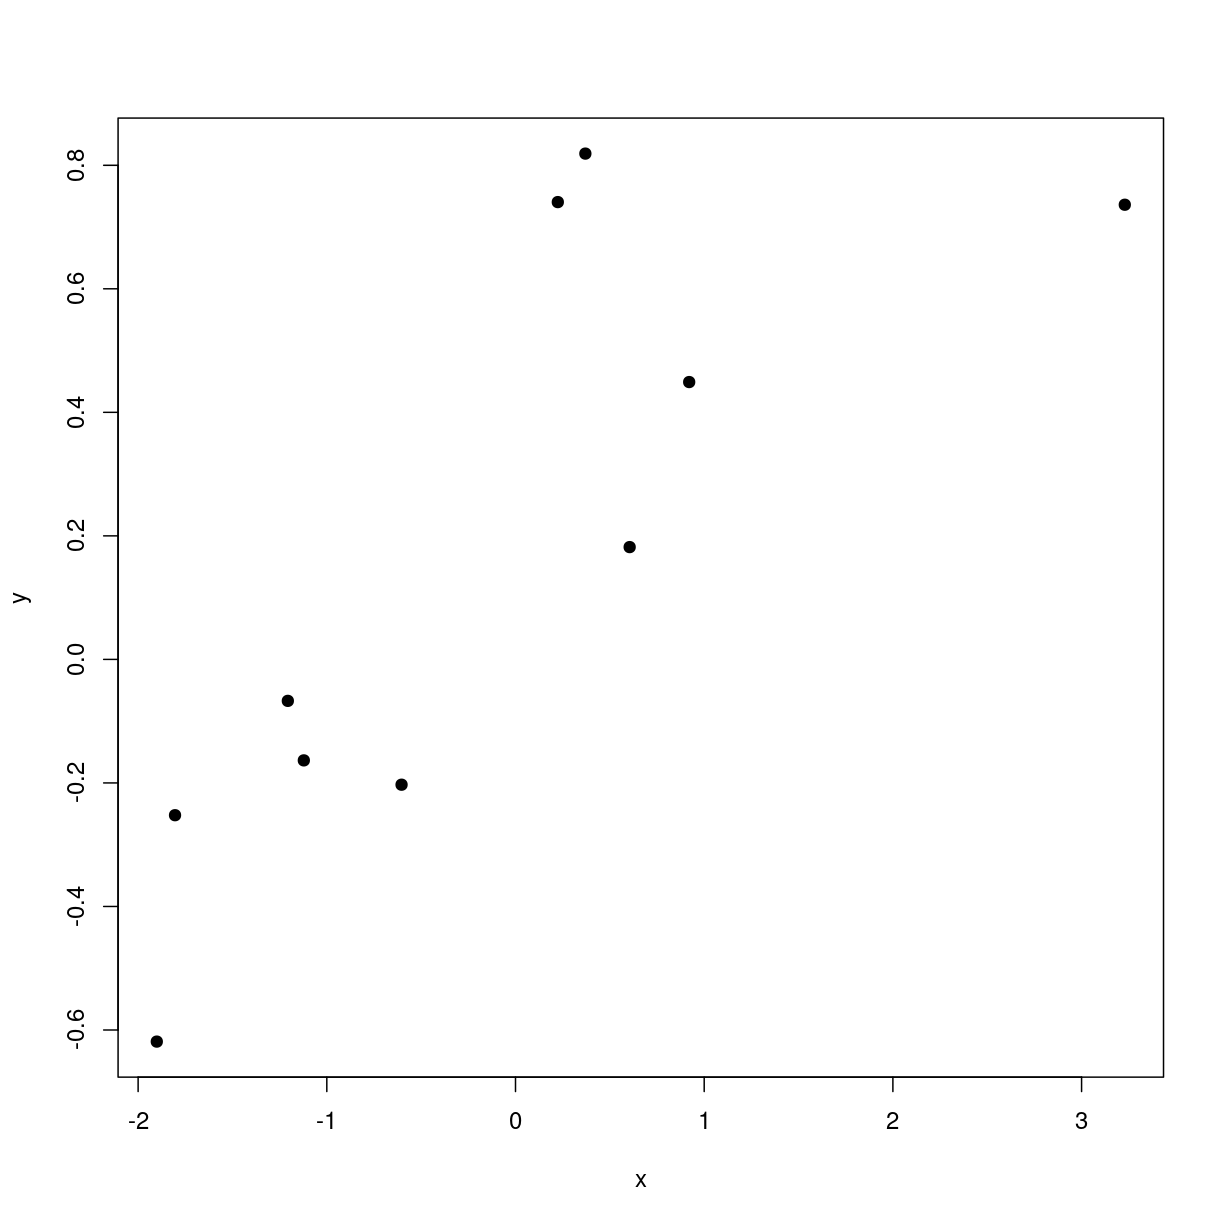
\includegraphics[width=0.5\textwidth]{/home/runner/work/high-dimensional-stats-r/high-dimensional-stats-r/fig/rmd-02-unnamed-chunk-9-1}



\end{frame}

\begin{frame}{plot of chunk unnamed-chunk-10}
\protect\hypertarget{plot-of-chunk-unnamed-chunk-10}{}

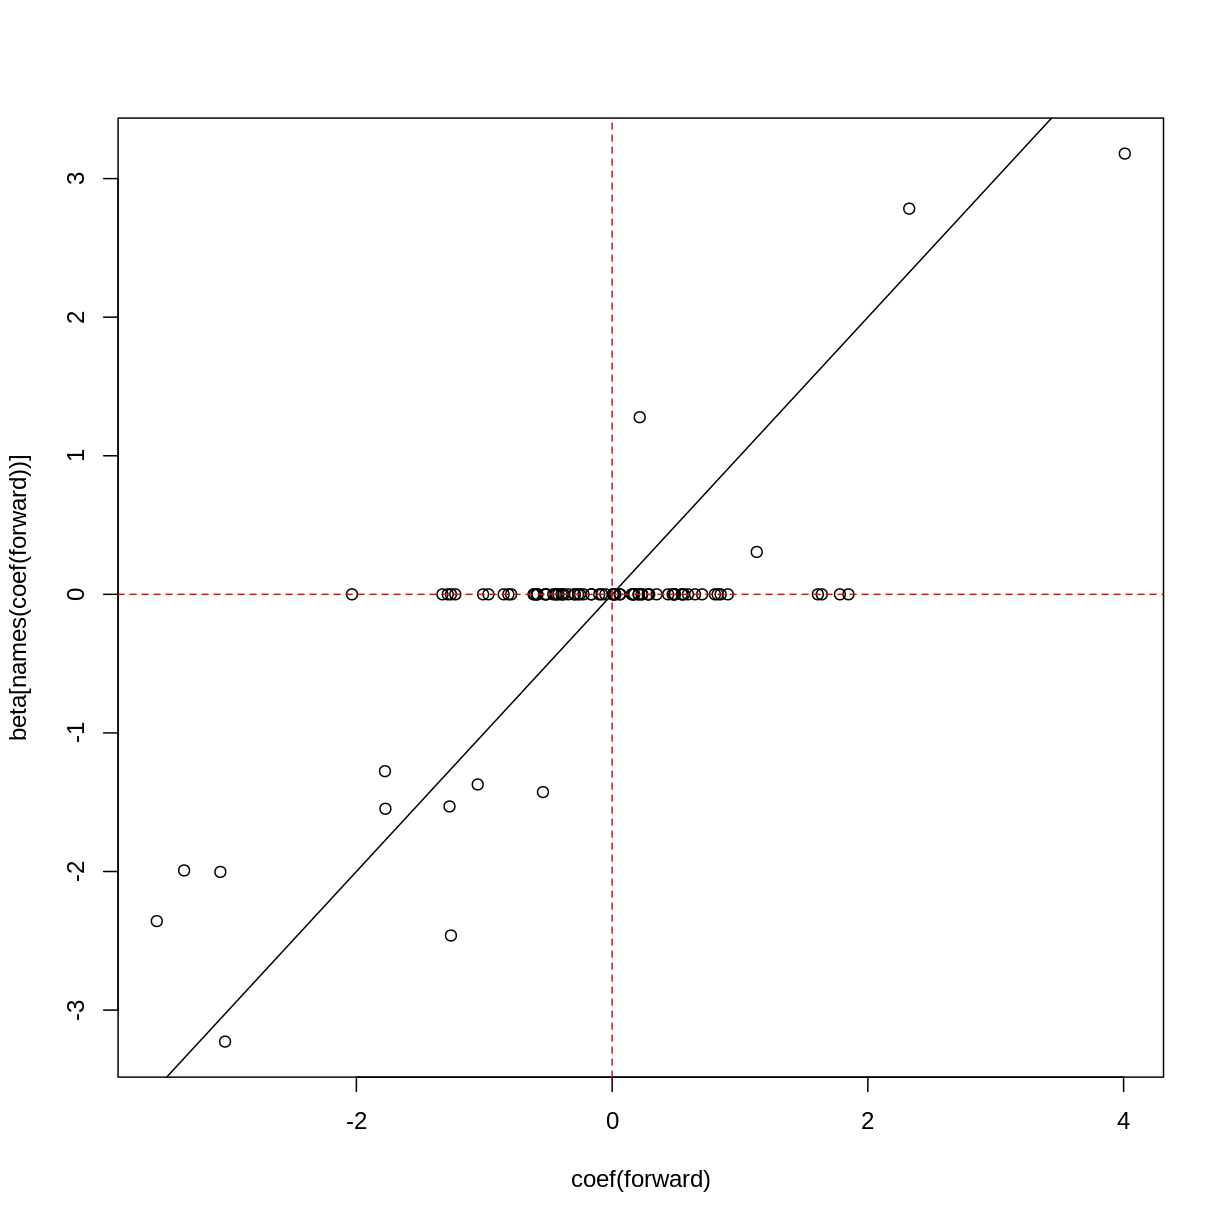
\includegraphics[width=0.5\textwidth]{/home/runner/work/high-dimensional-stats-r/high-dimensional-stats-r/fig/rmd-02-unnamed-chunk-10-1}



\end{frame}

\begin{frame}{plot of chunk unnamed-chunk-11}
\protect\hypertarget{plot-of-chunk-unnamed-chunk-11}{}

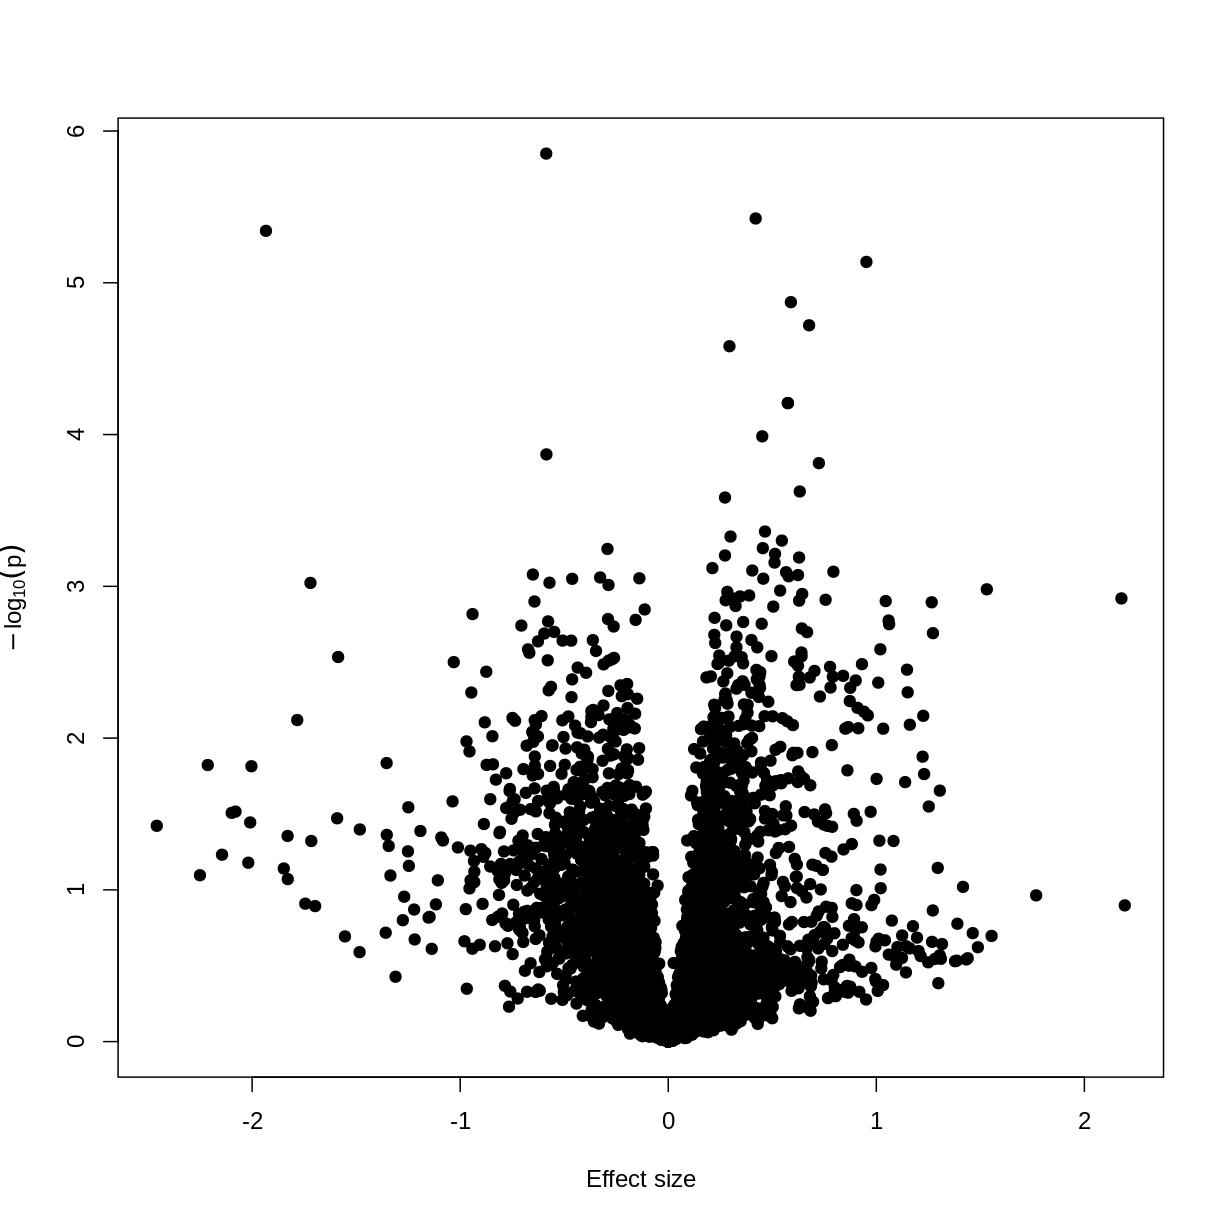
\includegraphics[width=0.5\textwidth]{/home/runner/work/high-dimensional-stats-r/high-dimensional-stats-r/fig/rmd-02-unnamed-chunk-11-1}



\end{frame}

\begin{frame}{plot of chunk unnamed-chunk-12}
\protect\hypertarget{plot-of-chunk-unnamed-chunk-12}{}

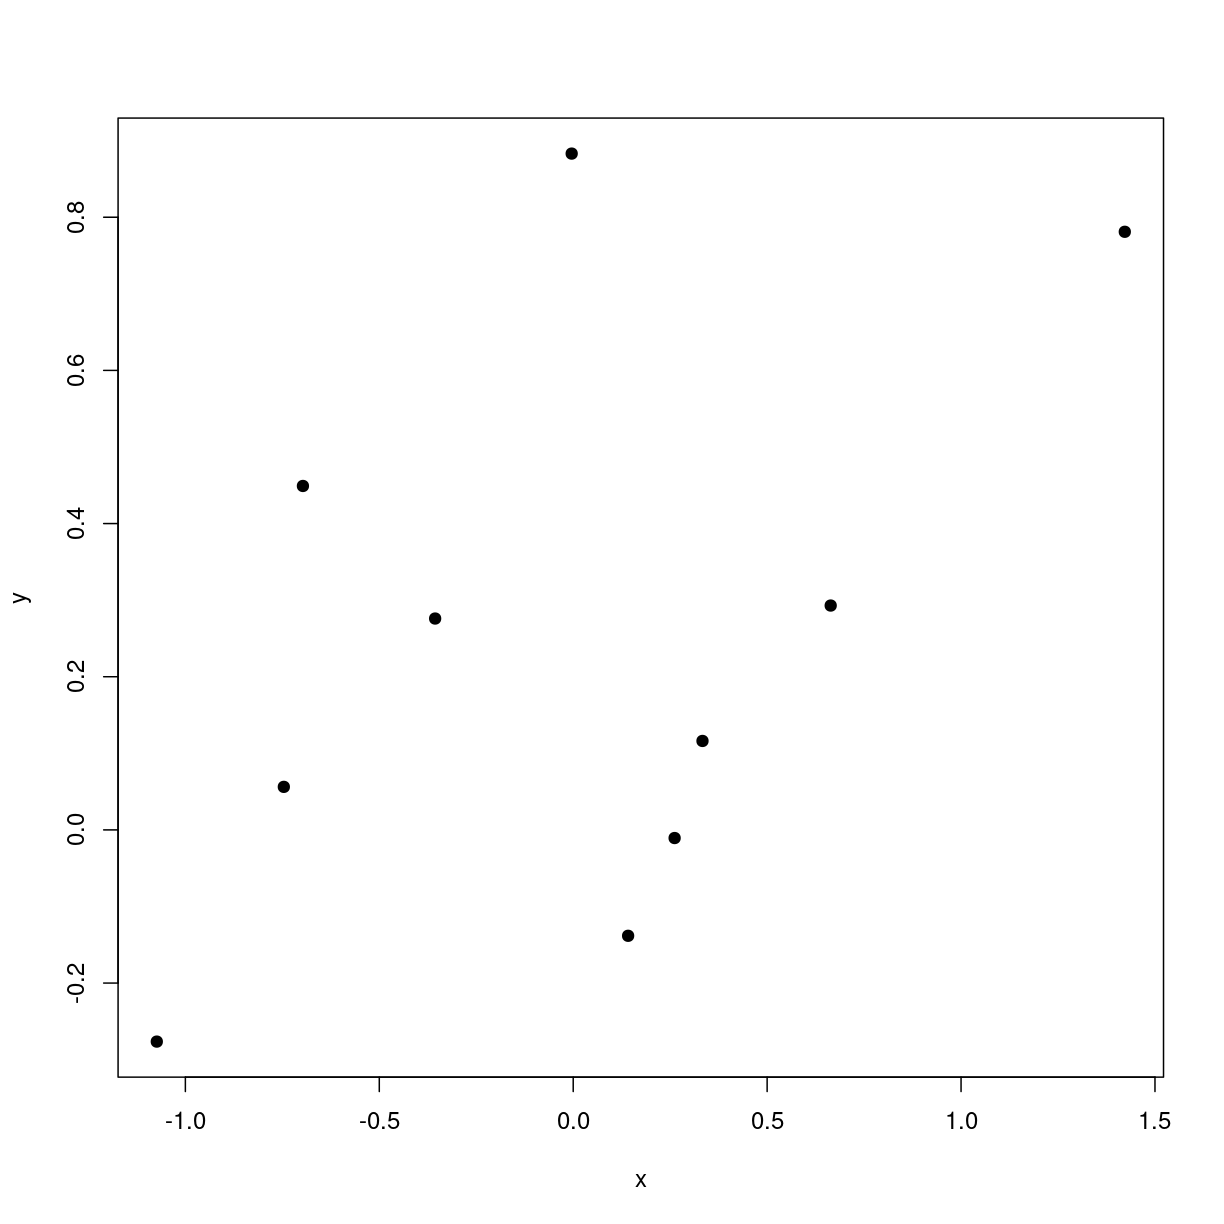
\includegraphics[width=0.5\textwidth]{/home/runner/work/high-dimensional-stats-r/high-dimensional-stats-r/fig/rmd-02-unnamed-chunk-12-1}



\end{frame}

\begin{frame}{plot of chunk unnamed-chunk-13}
\protect\hypertarget{plot-of-chunk-unnamed-chunk-13}{}

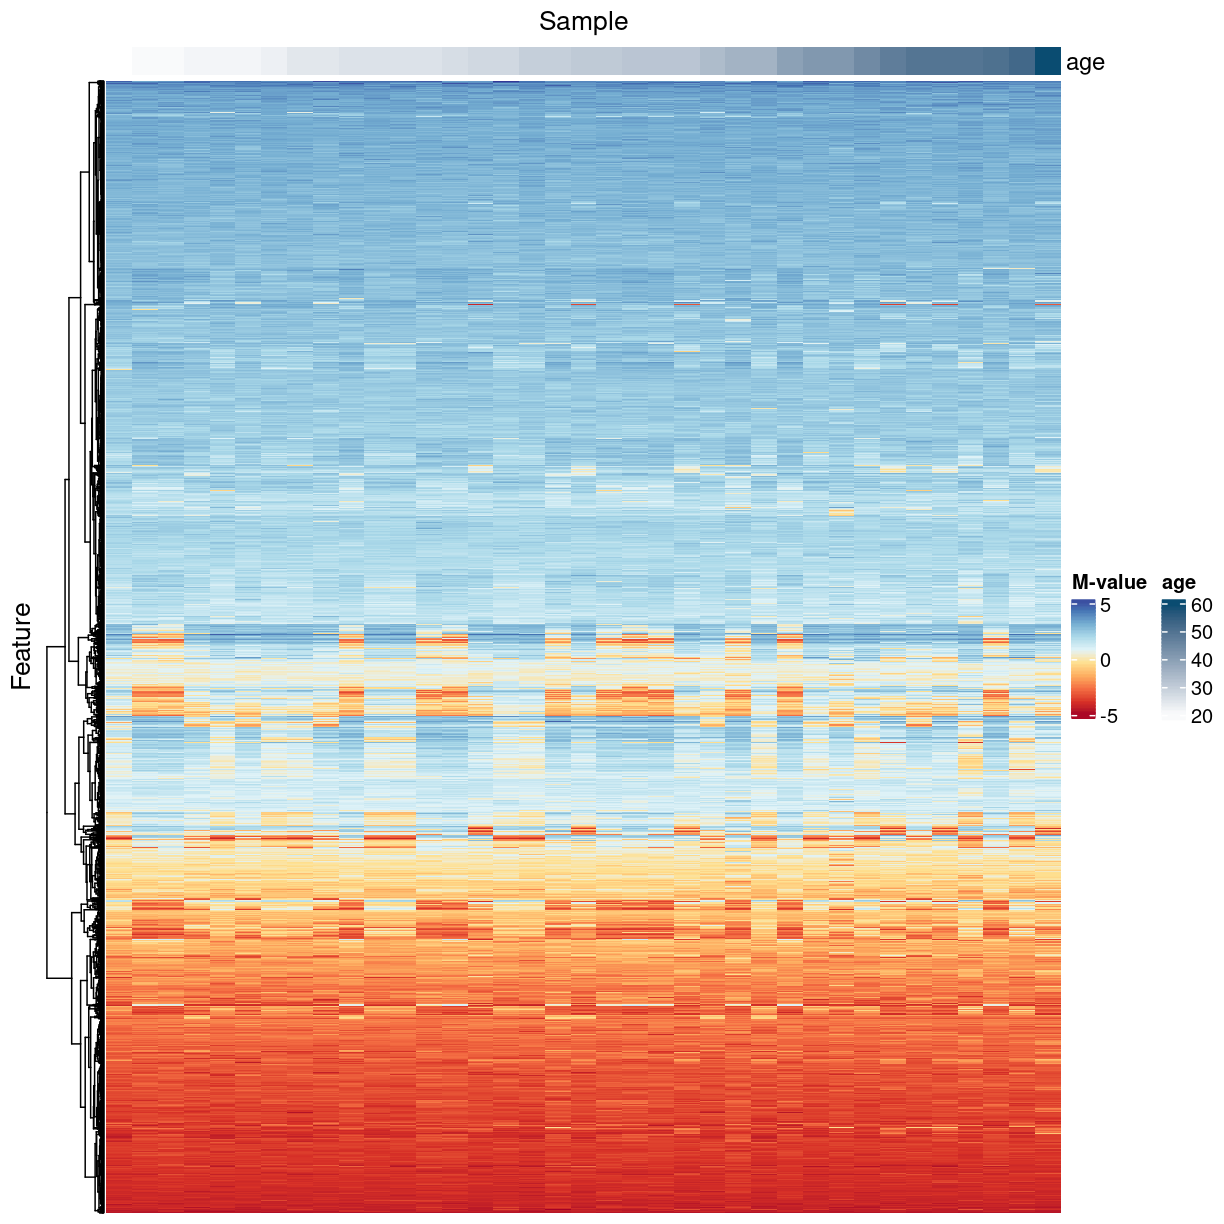
\includegraphics[width=0.5\textwidth]{/home/runner/work/high-dimensional-stats-r/high-dimensional-stats-r/fig/rmd-02-unnamed-chunk-13-1}



\end{frame}

\begin{frame}{plot of chunk unnamed-chunk-14}
\protect\hypertarget{plot-of-chunk-unnamed-chunk-14}{}

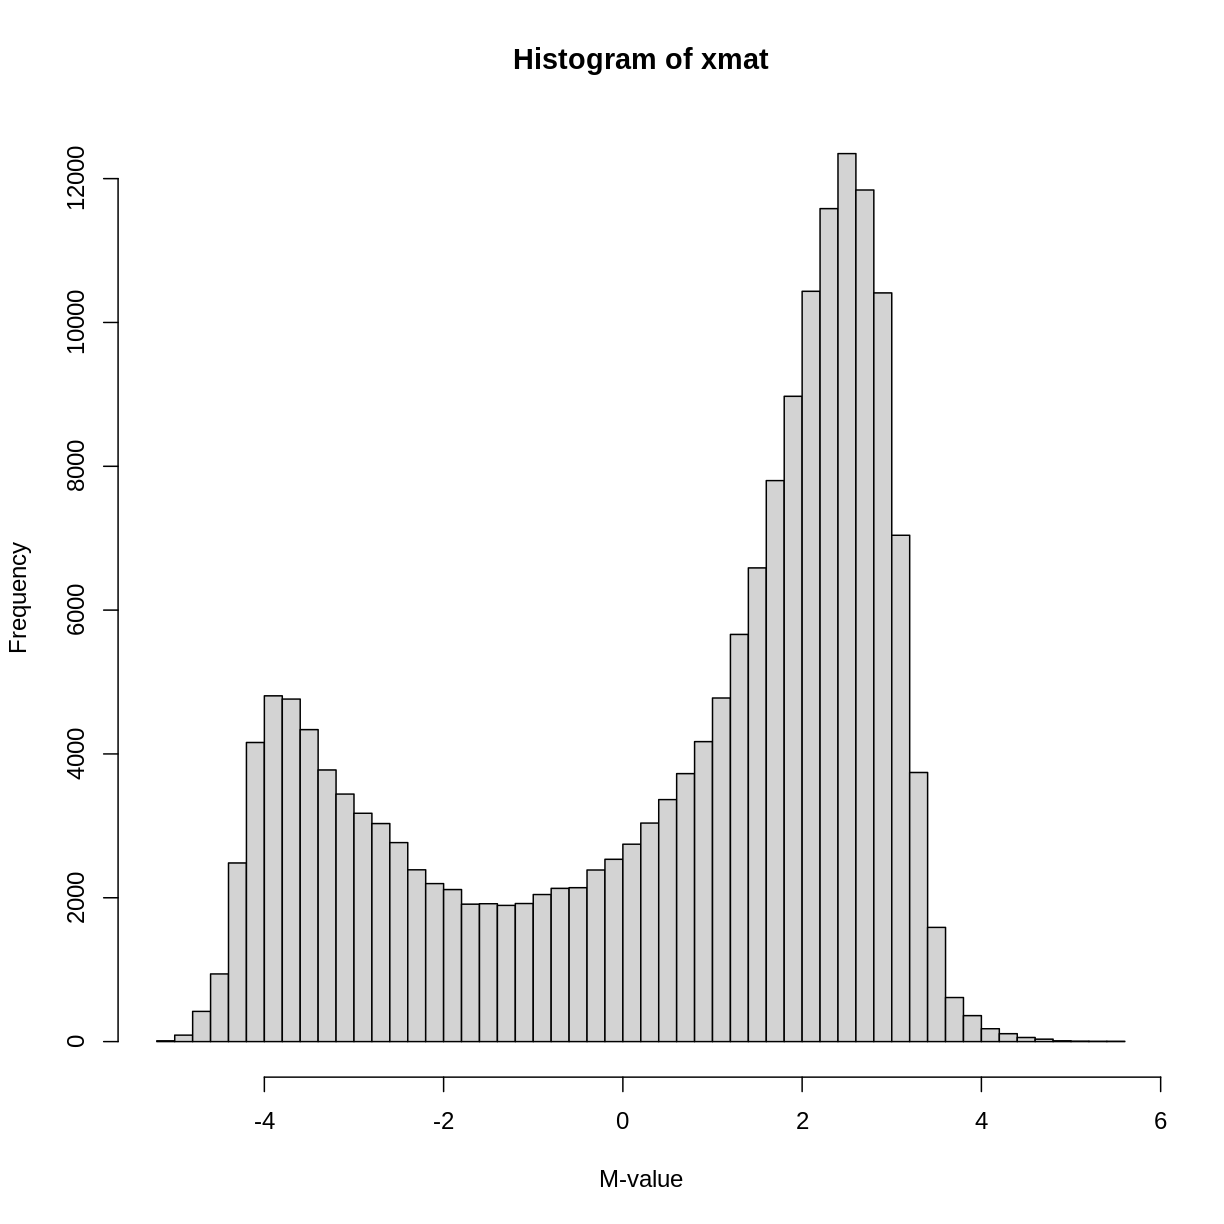
\includegraphics[width=0.5\textwidth]{/home/runner/work/high-dimensional-stats-r/high-dimensional-stats-r/fig/rmd-02-unnamed-chunk-14-1}



\end{frame}

\begin{frame}{plot of chunk unnamed-chunk-19}
\protect\hypertarget{plot-of-chunk-unnamed-chunk-19}{}

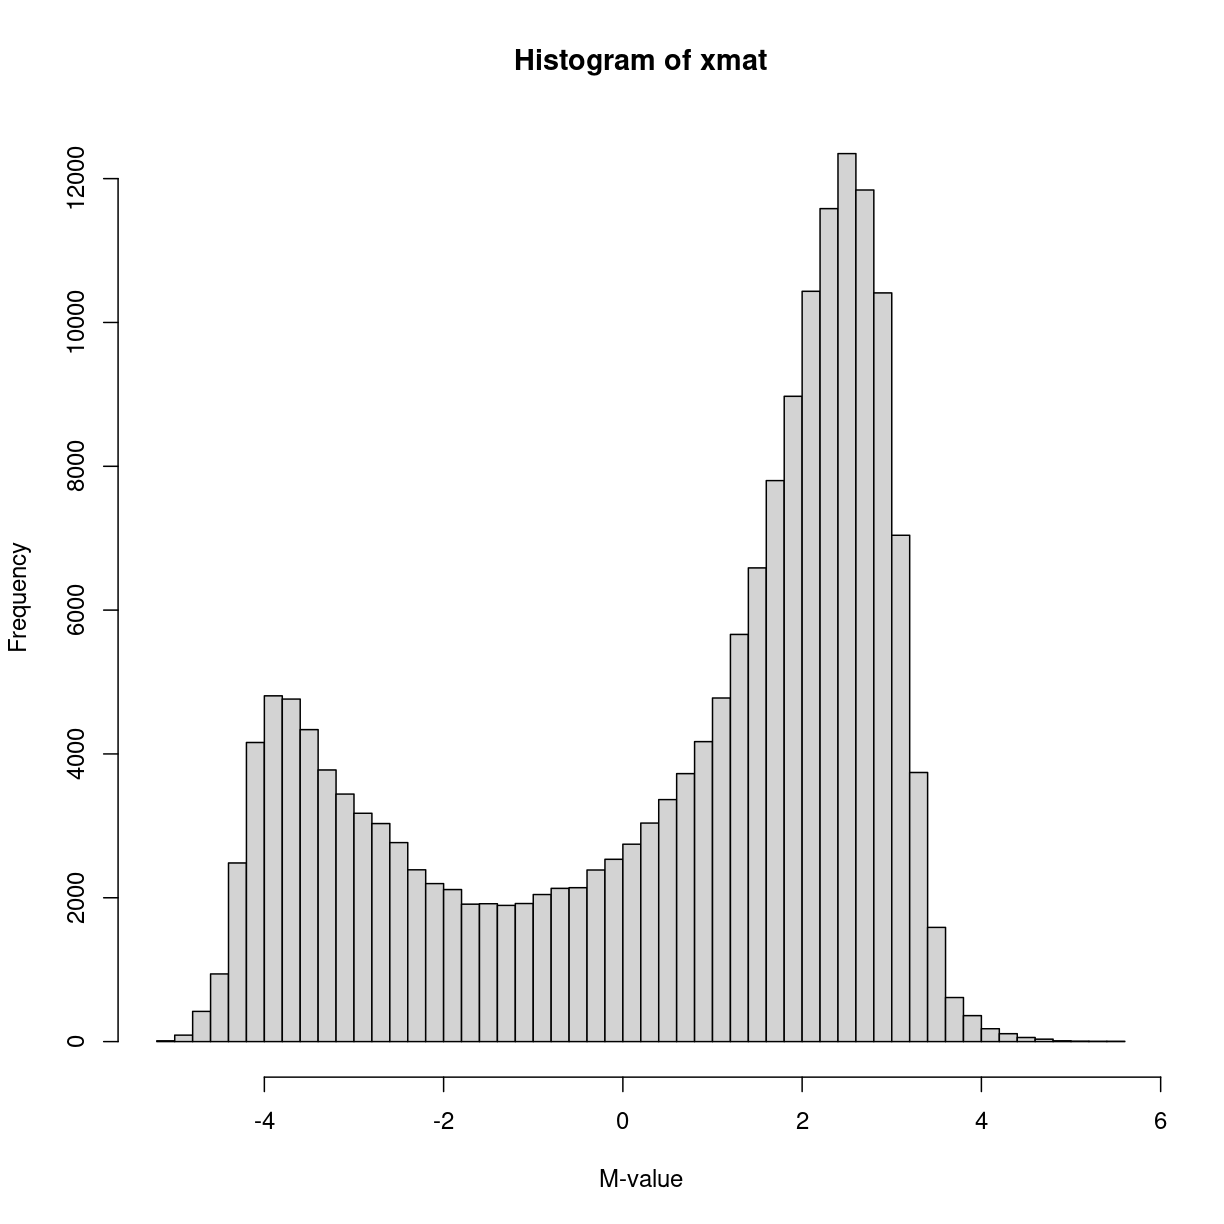
\includegraphics[width=0.5\textwidth]{/home/runner/work/high-dimensional-stats-r/high-dimensional-stats-r/fig/rmd-02-unnamed-chunk-19-1}



\end{frame}

\begin{frame}{plot of chunk unnamed-chunk-21}
\protect\hypertarget{plot-of-chunk-unnamed-chunk-21}{}

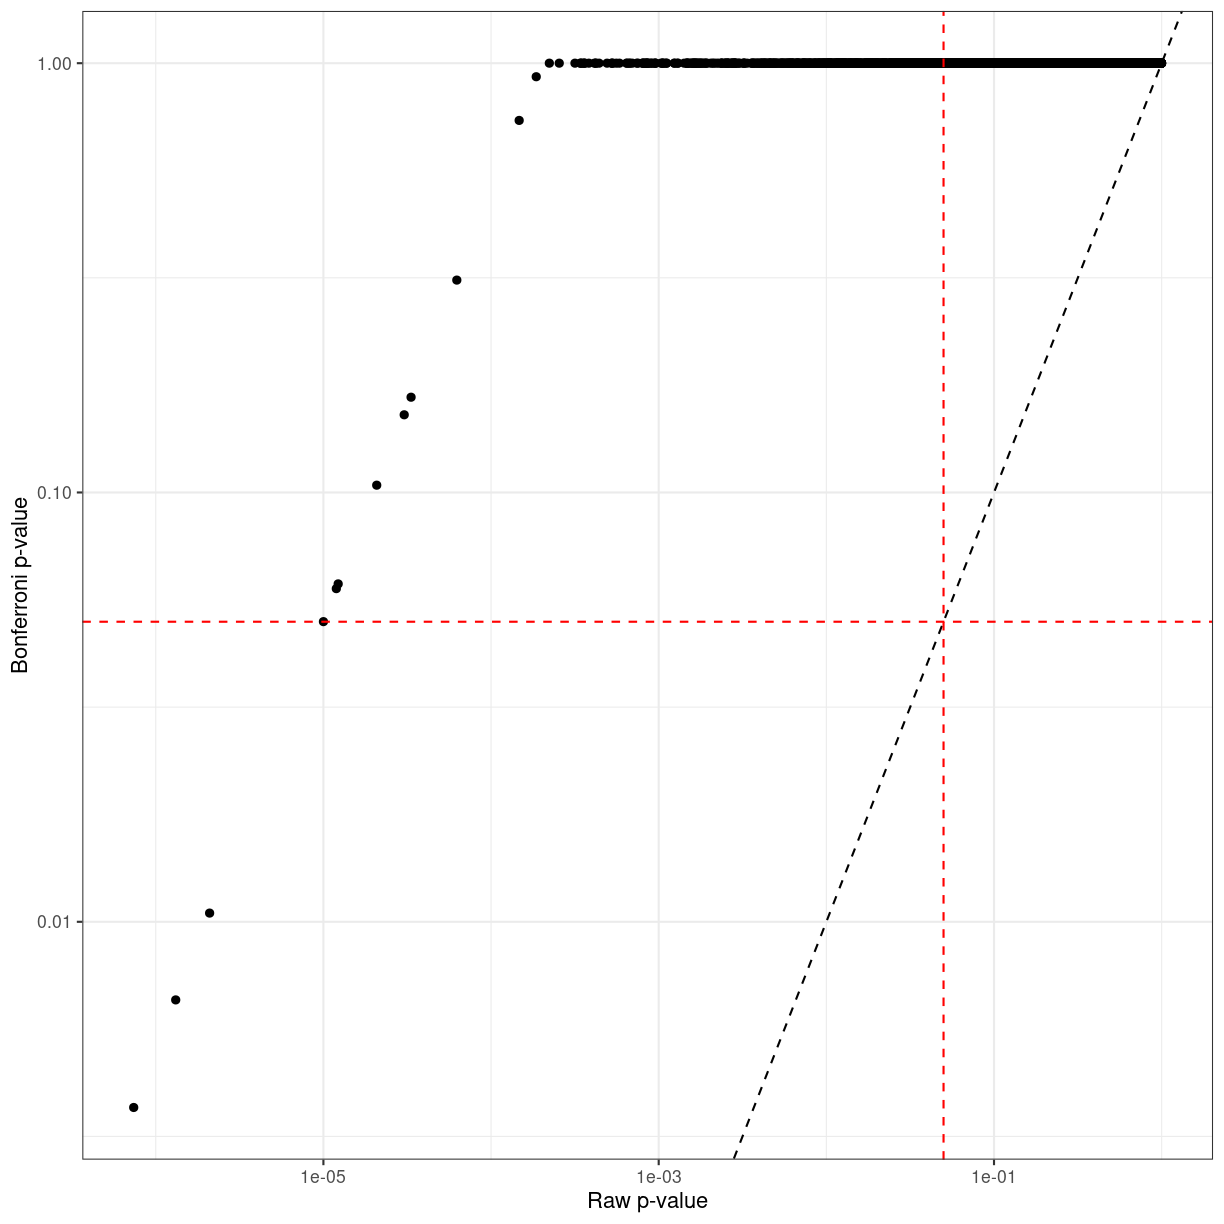
\includegraphics[width=0.5\textwidth]{/home/runner/work/high-dimensional-stats-r/high-dimensional-stats-r/fig/rmd-02-unnamed-chunk-21-1}



\end{frame}

\begin{frame}{Plot of -log10(p) against effect size estimates for a
regression of age against methylation level for each feature in the
data.}
\protect\hypertarget{plot-of--log10p-against-effect-size-estimates-for-a-regression-of-age-against-methylation-level-for-each-feature-in-the-data.}{}

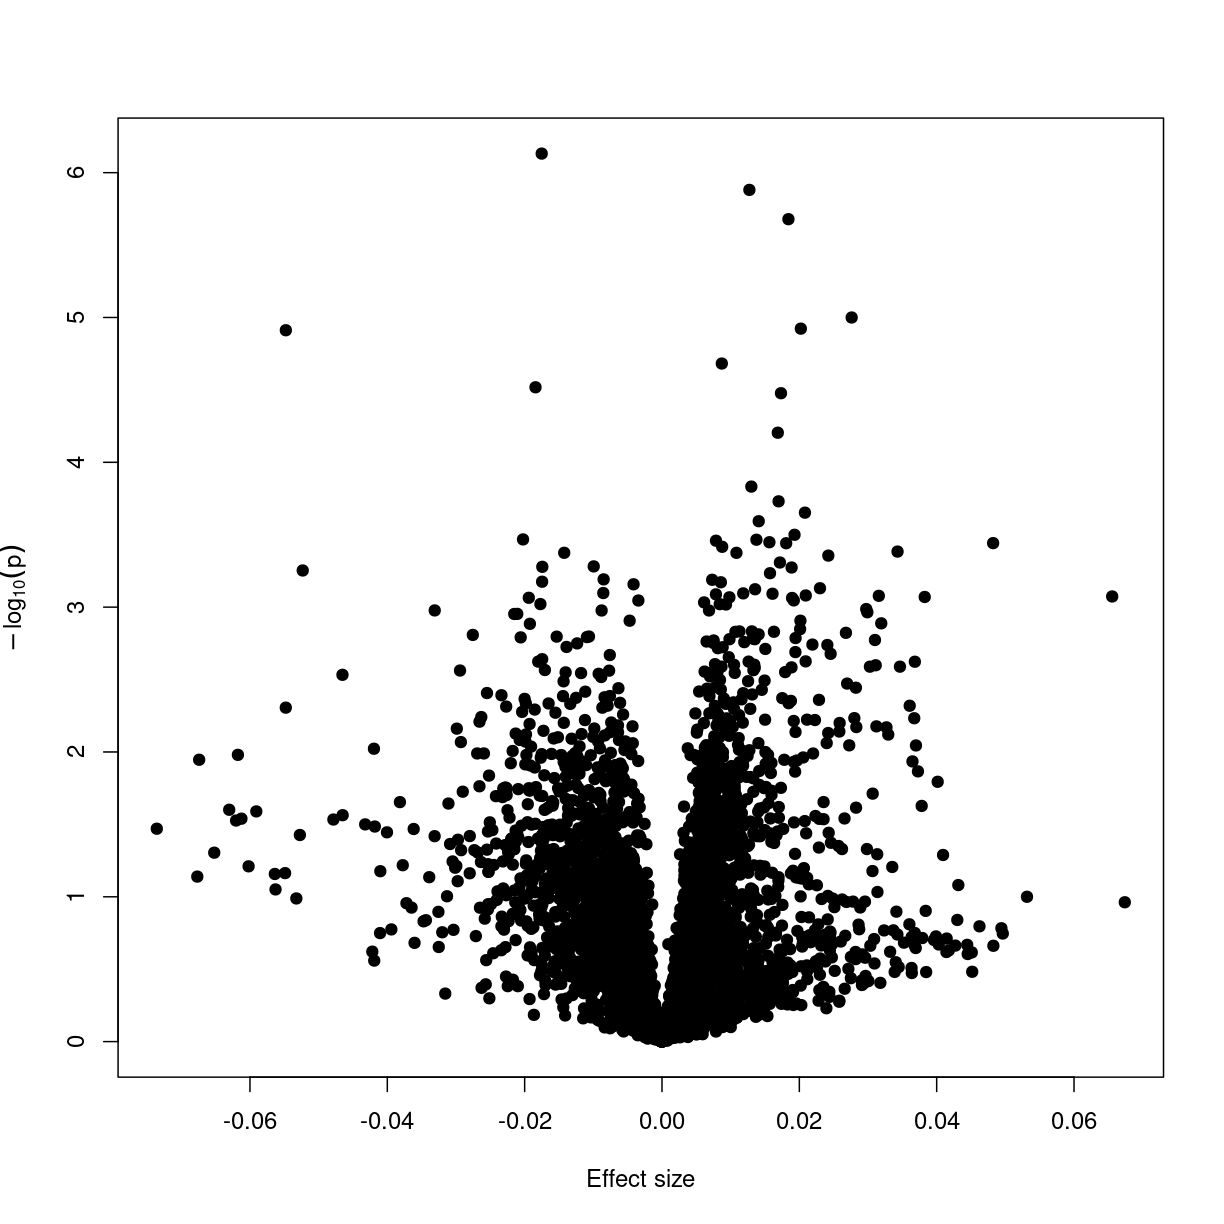
\includegraphics[width=0.5\textwidth]{/home/runner/work/high-dimensional-stats-r/high-dimensional-stats-r/fig/rmd-02-unnamed-chunk-28-1}



\end{frame}

\begin{frame}{plot of chunk unnamed-chunk-29}
\protect\hypertarget{plot-of-chunk-unnamed-chunk-29}{}

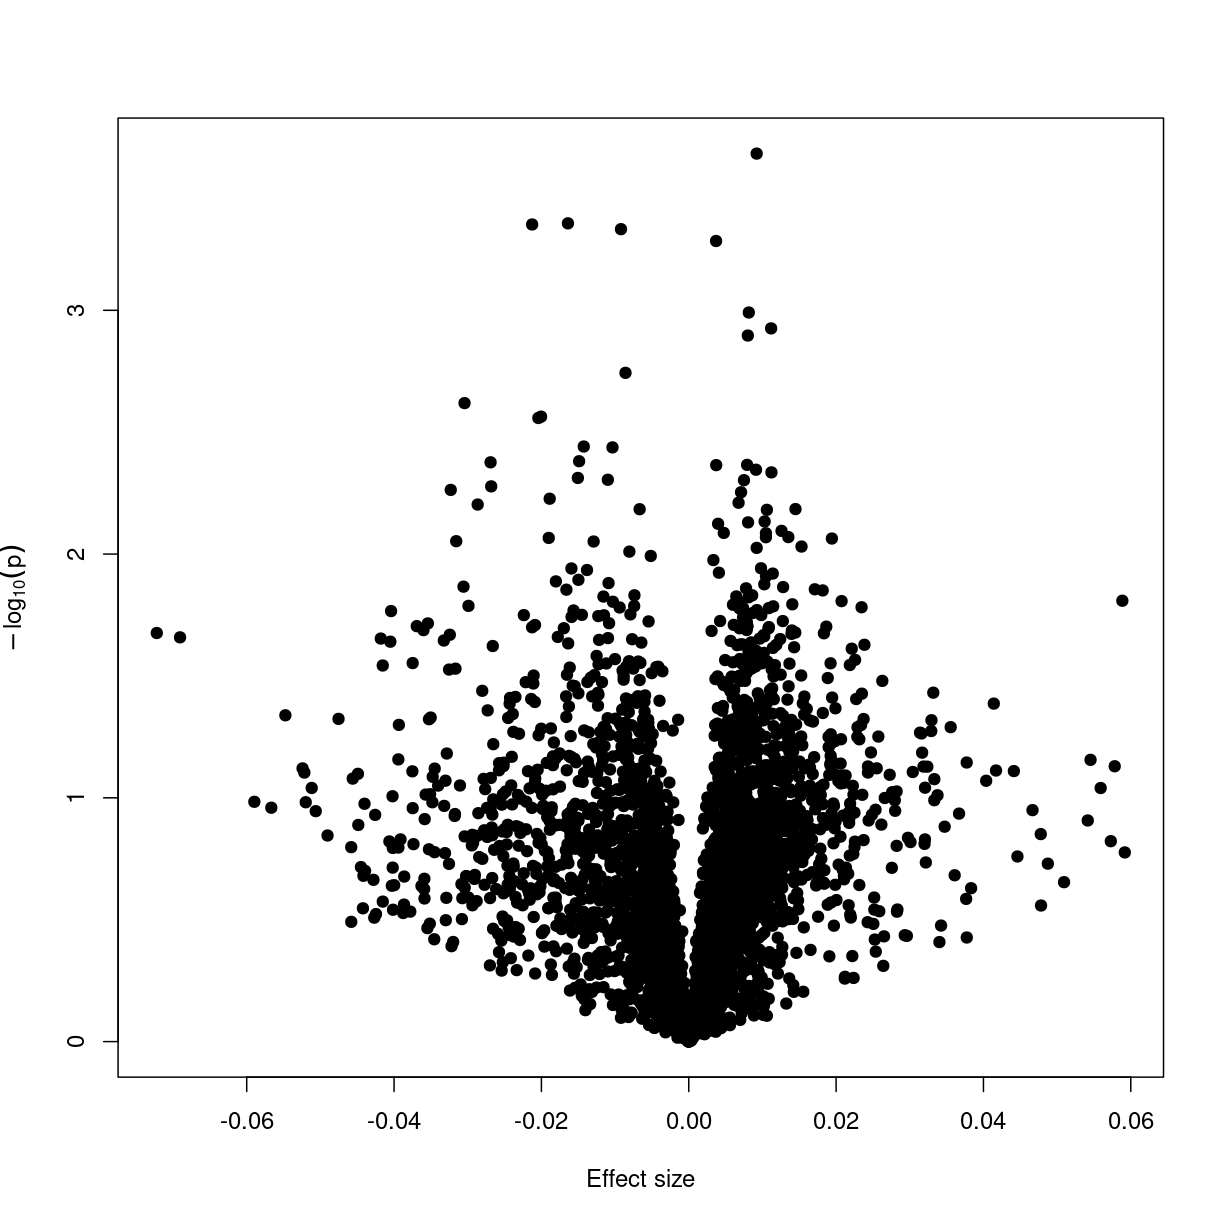
\includegraphics[width=0.5\textwidth]{/home/runner/work/high-dimensional-stats-r/high-dimensional-stats-r/fig/rmd-02-unnamed-chunk-29-1}



\end{frame}

\begin{frame}{plot of chunk unnamed-chunk-30}
\protect\hypertarget{plot-of-chunk-unnamed-chunk-30}{}

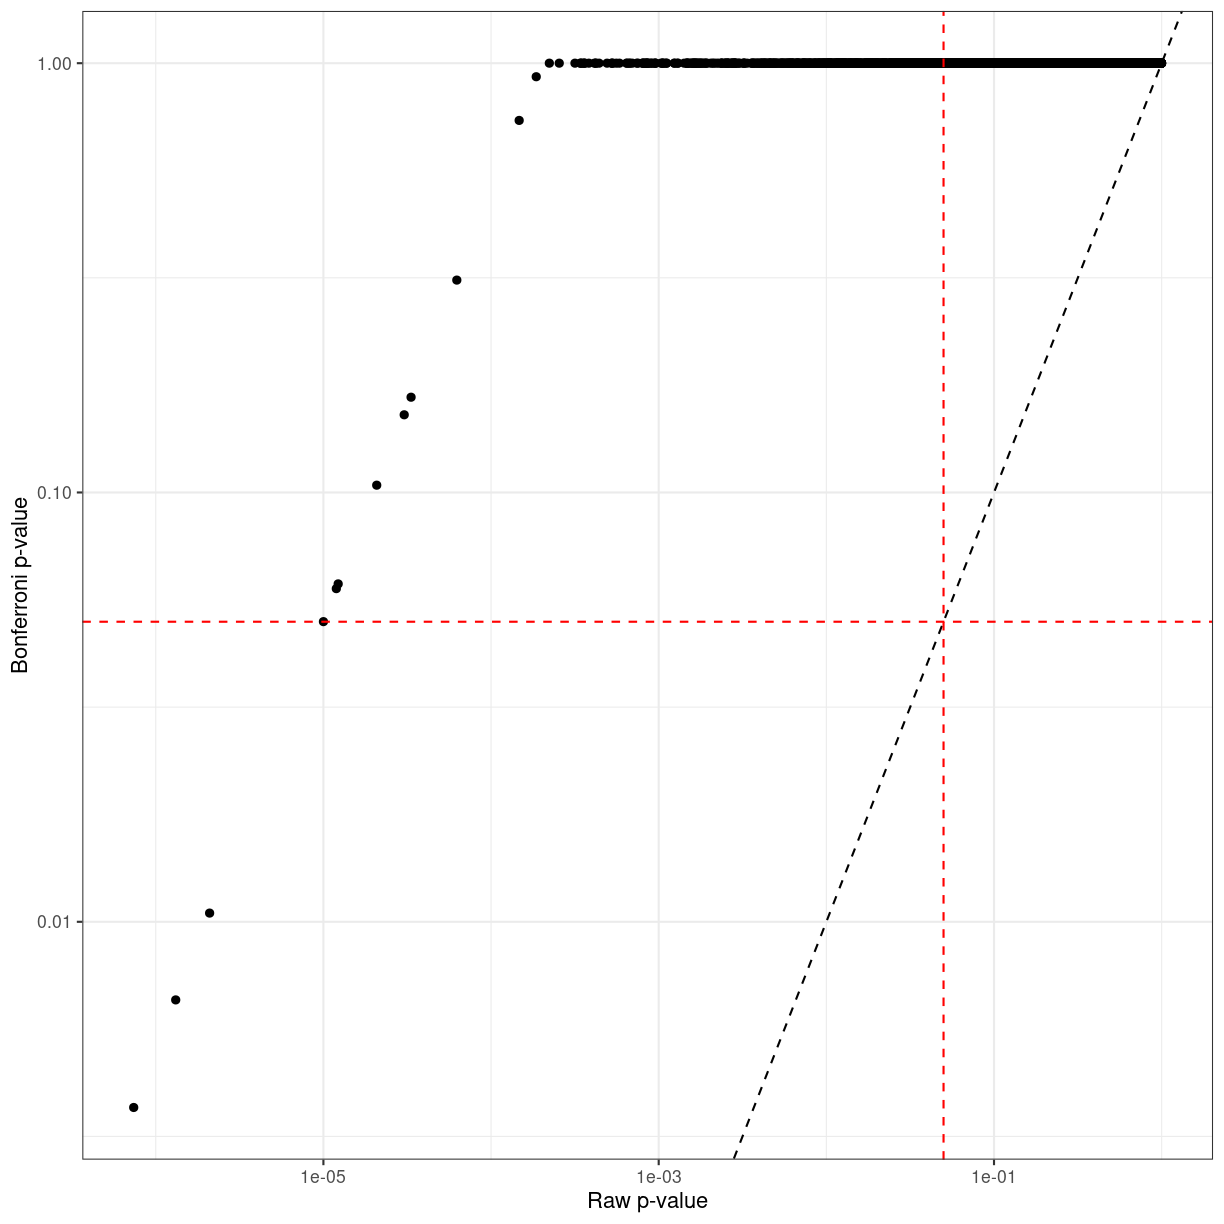
\includegraphics[width=0.5\textwidth]{/home/runner/work/high-dimensional-stats-r/high-dimensional-stats-r/fig/rmd-02-unnamed-chunk-30-1}



\end{frame}

\begin{frame}{plot of chunk unnamed-chunk-31}
\protect\hypertarget{plot-of-chunk-unnamed-chunk-31}{}

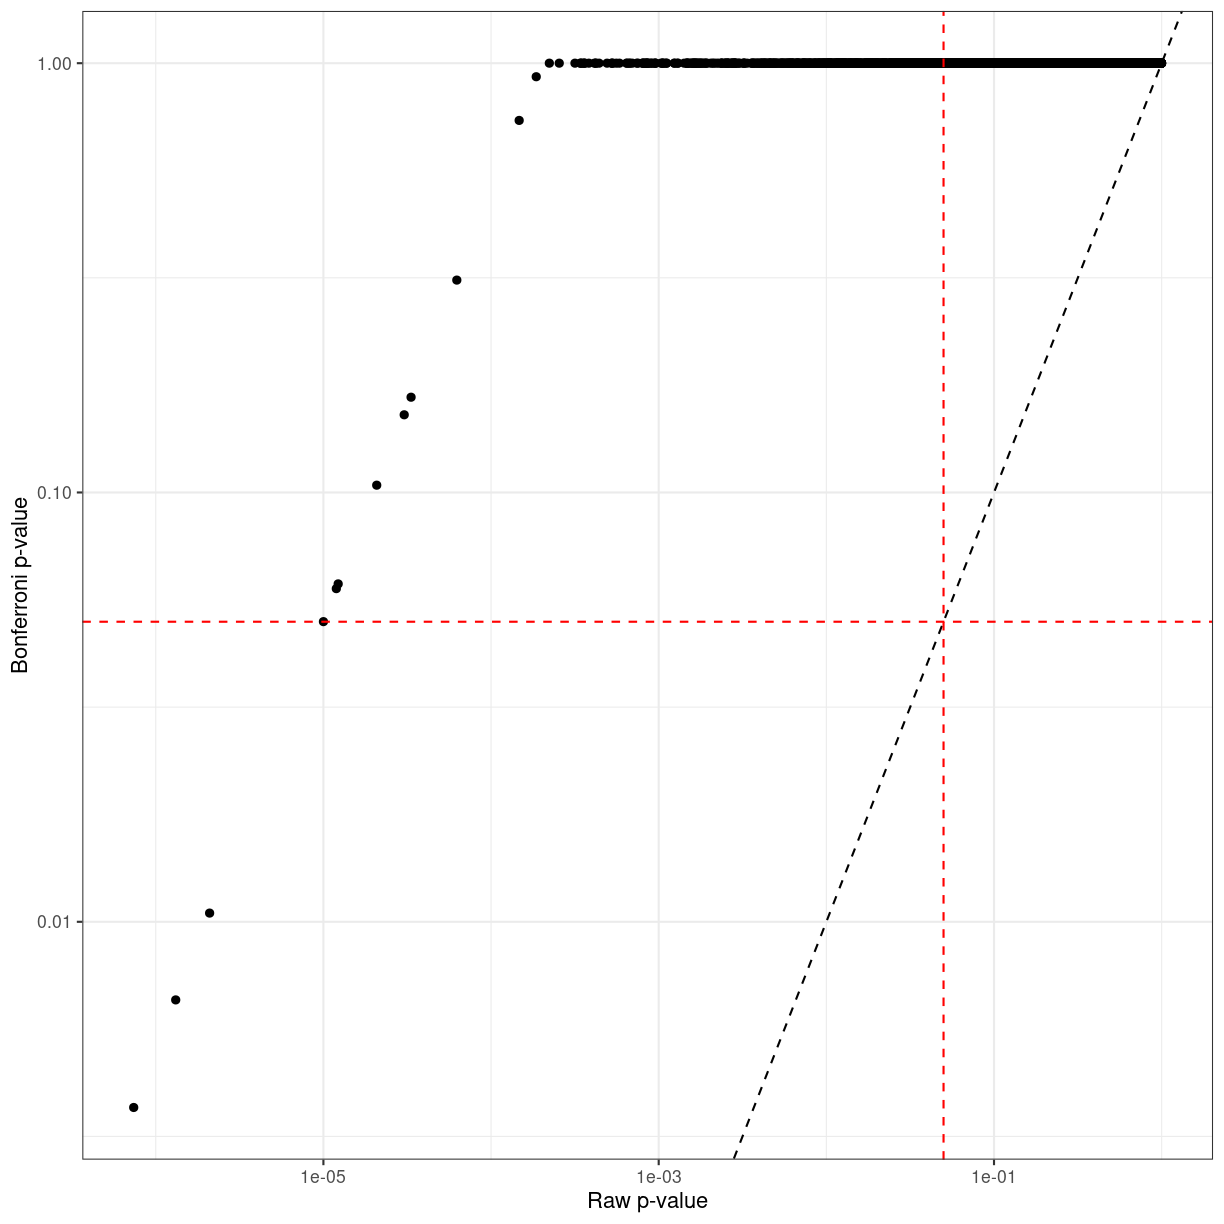
\includegraphics[width=0.5\textwidth]{/home/runner/work/high-dimensional-stats-r/high-dimensional-stats-r/fig/rmd-02-unnamed-chunk-31-1}



\end{frame}

\begin{frame}{plot of chunk unnamed-chunk-31}
\protect\hypertarget{plot-of-chunk-unnamed-chunk-31-1}{}

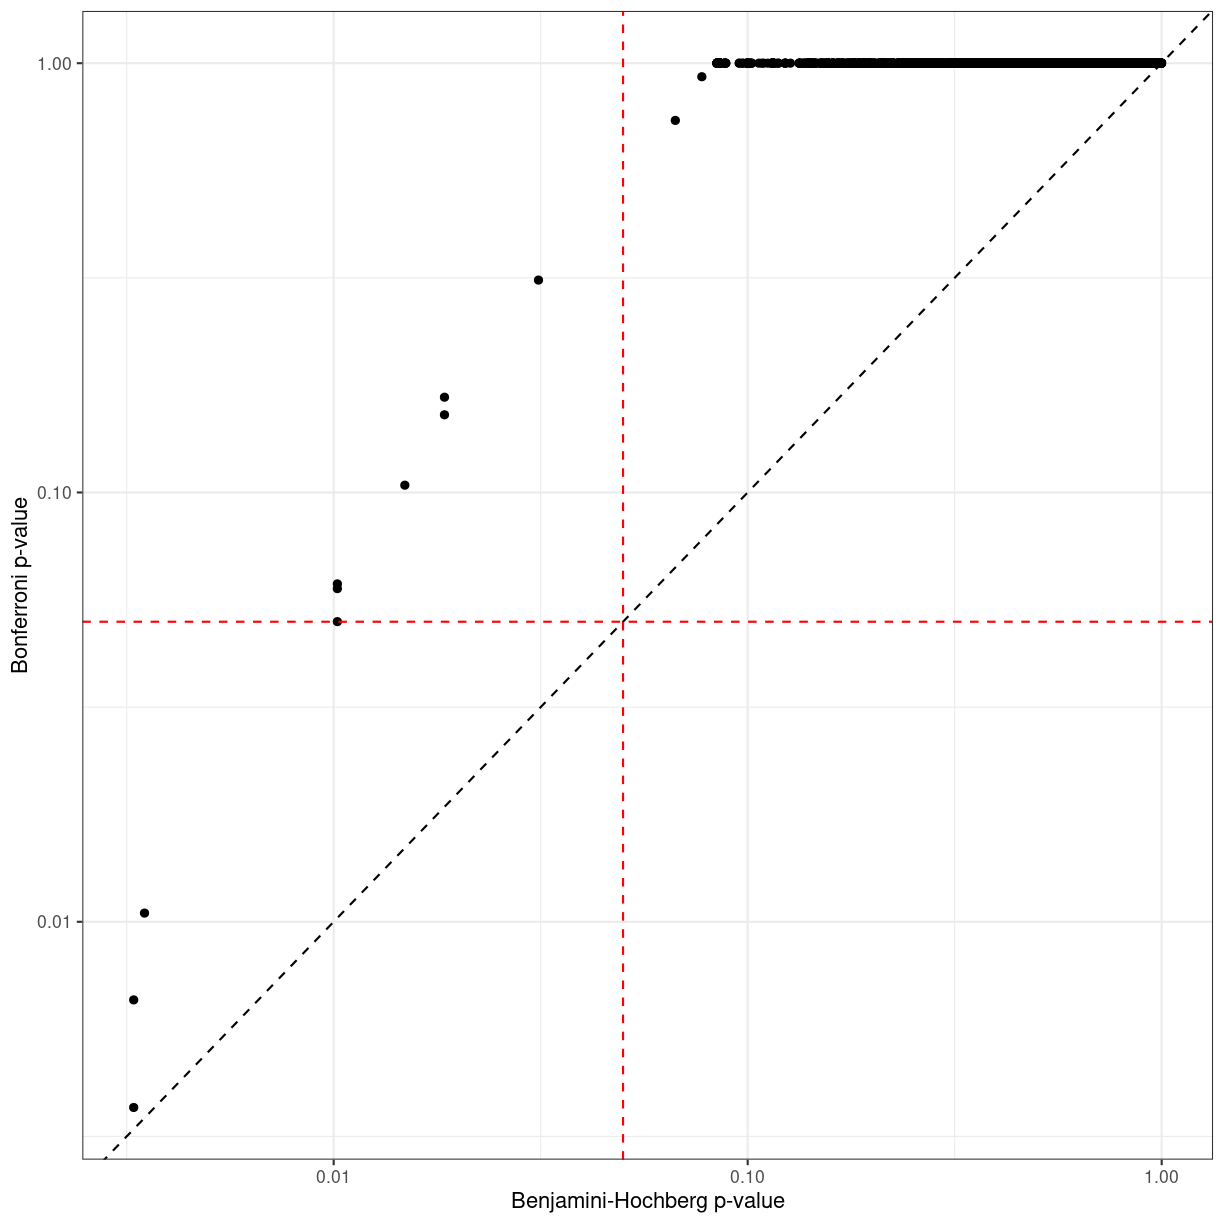
\includegraphics[width=0.5\textwidth]{/home/runner/work/high-dimensional-stats-r/high-dimensional-stats-r/fig/rmd-02-unnamed-chunk-31-2}



\end{frame}

\begin{frame}{plot of chunk unnamed-chunk-32}
\protect\hypertarget{plot-of-chunk-unnamed-chunk-32}{}

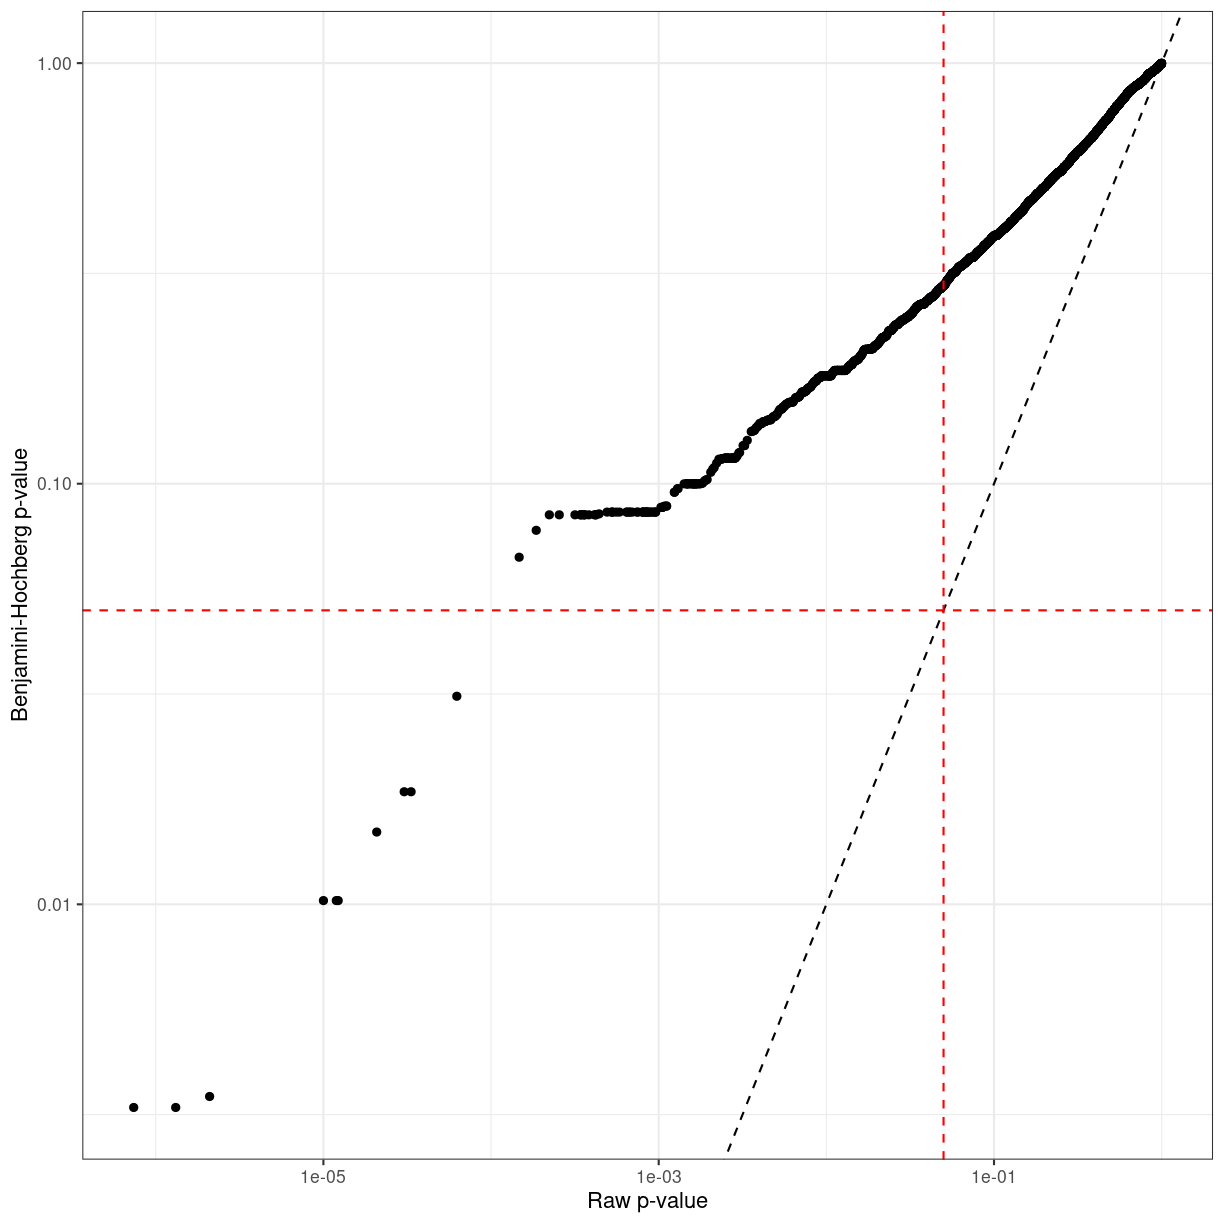
\includegraphics[width=0.5\textwidth]{/home/runner/work/high-dimensional-stats-r/high-dimensional-stats-r/fig/rmd-02-unnamed-chunk-32-1}



\end{frame}

\begin{frame}{plot of chunk unnamed-chunk-34}
\protect\hypertarget{plot-of-chunk-unnamed-chunk-34}{}

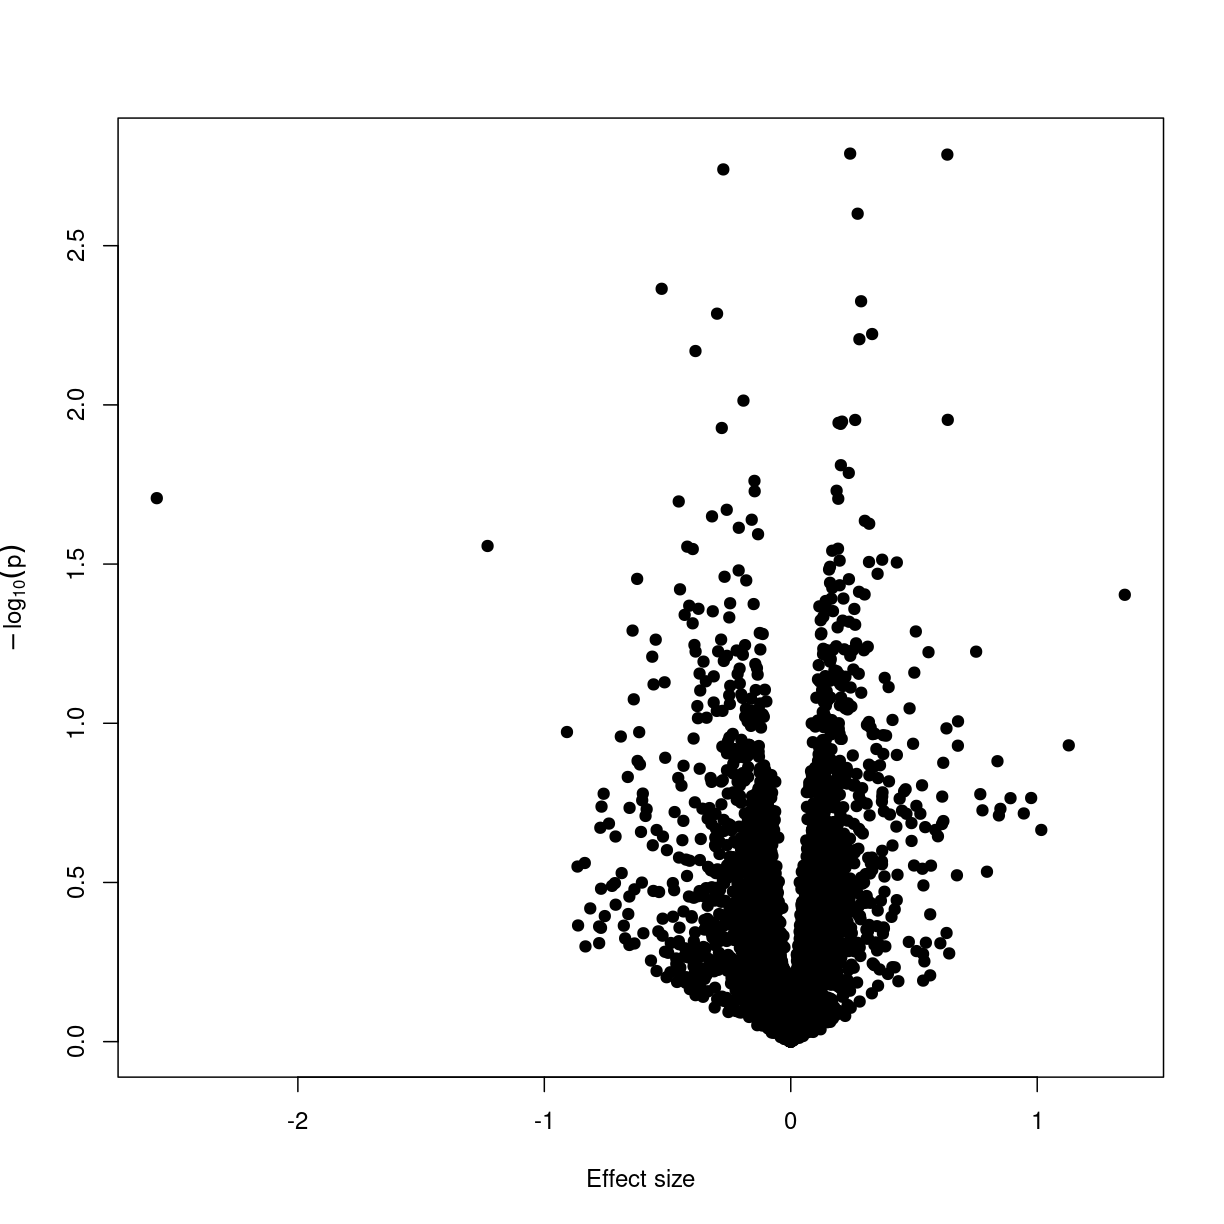
\includegraphics[width=0.5\textwidth]{/home/runner/work/high-dimensional-stats-r/high-dimensional-stats-r/fig/rmd-02-unnamed-chunk-34-1}



\end{frame}

\end{document}
